\documentclass{article}
\usepackage[utf8]{inputenc}
\usepackage[T1]{fontenc}
\usepackage[MeX]{polski}
\usepackage{enumerate}
\usepackage{courier}
\usepackage{graphicx}


\title{Bezpieczeństwo Komputerowe - lista 1, zadanie 1}
\author{Mateusz Kalinowski}
\begin{document}
\maketitle
\newpage
\section{Opis:}
Najwięcej urządzeń łączyło się do udostępnianych sieci o nazwach sieci znanych i zaufanych miejsc, przykładowo \textit{KFC Wifi, McDonalds Wifi, PasażGrunwaldzki Wifi}. Do innych sieci, których nazwy nie wzbudzały zaufania użytkownicy łączyli się rzadko lub wcale, przykładowo \textit{Iphone(Mateusz), darmoweWifi}. Najwięcej jednak było użytkowników w sieciach ogólnodostępnych udostępnianych przez miejsca publiczne, miały one najlepszy zasięg i największe zaufanie. 
\\
\\
Do analizy statystyk bierzemy najbardziej interesujący plik z największą ilością wejść, nasłuchiwanie miało miejsce pd ogólnodostępną siecią w Pasażu Grunwaldzkim.
\section{Statystyki:}

\begin{enumerate}[] 
\item \textbf{Liczba użytkowników} - liczbę użytkowników w danej sieci podczas danego nasłuchiwania można uzyskać łatwo przy pomocy przefiltrowania protokołu dns.
Dokładne numery ip uzytkowników możemy uzyskać w poniższy sposób:
\\
\\
Komenda: 
\begin{small}\texttt{tshark -r file.pcap -T fields -e ip.src -Y "dns.flags.response eq 0" | sort | uniq}
\end{small}
\\
\\
Aby dostać dokładną liczbę należy przepuścić output przez potok wc -l. Z nasłuchiwaną siecią połączonych było 12 użytkowników.
\\
\item \textbf{Odwiedzane strony} - samą informację o stronach na które wchodzili użytkownicy możemy otrzymać również poprzez przefiltrowanie protokołów DNS. Czyli po prostu sprawdzenie jakie adresy ip obługiwane były przez serwery DNS podczas nasłuchiwania.
 \\
\\
Komenda: 
\begin{small}\texttt{tshark -r file.pcap -T fields -e dns.qry.name -Y "dns.flags.response eq 0" | sort | uniq}
\end{small}
\\
\\
Komenda ta zwraca unikatową listę stron, z którymi łączyli sie użytkownicy. Możemy zauważyć na jak różnorodne strony wchodzili użytkownicy. Wśród wyszukiwań możemy zauważyć najpopularniejsze strony takie jak \textit{youtube.com, google.com, facebook.com, instagram.com} jak również różnego rodzaju strony z newsami i wiadomościami takie jak \textit{wprost.com, weszło.com, interia.pl}, można również zauważyć dość nietypowe i mniej popularne strony jak \textit{maxior.pl, umk.pl,...}
\\
\\
\item \textbf{Wykorzystane protokoły i usługi} - Większość użytkowników używała protokołu HTTPS czyli wersji HTTP zabezpieczonej protokołem TLS, przez takie połączenie nie udało sie bezpośrednio dostać do danych użytkowników. Praktycznie wszystkie strony obecnie używają protokołu HTTPS, zdarzają się jednak strony które używają jeszcze niezabezpieczonej wersji HTTP. W takie sytuacji jawne są hasła użytkowników przesyłane metodą HTTP POST, czy ciasteczka z id sesji przesyłane podczas żądania HTTP GET. Można również przejrzeć wszystkie zdjęcia i filmiki pobierane przez użytkowników.
\\
\\
\begin{table}[h]
\def\arraystretch{1.5}%
\begin{tabular}{|c|c|c|}
\hline
strona        & możliwe do uzyskania dane               & używany protokół \\ \hline
gry.pl        & id sesji z ciasteczek, dane logowania   & HTTP             \\ \hline
giercownia.pl & id sesji z ciasteczek                   & HTTP             \\ \hline
weszło.com    & dane z rejestracji, logowania, id sesji & HTTP             \\ \hline
soso.com      & wyszukiwane frazy                       & HTTP             \\ \hline
facebook.com  & -                                       & HTTPS            \\ \hline
google.com    & -                                       & HTTPS            \\ \hline
...           & -                                       &                  \\ \hline
\end{tabular}
\end{table}
\\
\\
Ponadto można znaleźć chińską przeglądarkę \textit{soso.com} korzystającą dalej z protokołu HTTP w której można przejrzeć szukane frazy filtrem \begin{small}\texttt{http.host==soso.com}.
\end{small}
\\
\textbf{Lokalizacje serwerów} - Informacje z jakimi lokalizacjami łączyły sie komputery są łatwo dostępne w programie visual route, po wpisaniu nazwy wyszukiwanego hosta.
\end{enumerate}
  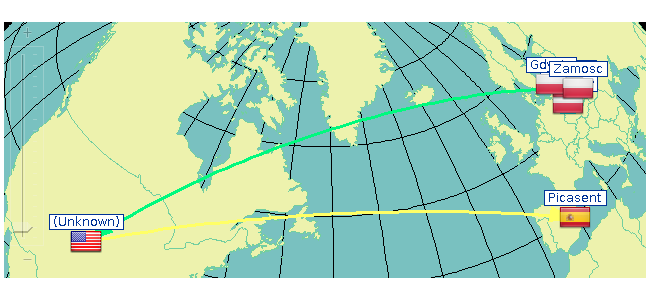
\includegraphics[width=\textwidth]{img2/weszlo.png}
\centering weszlo.com - polska strona sportowa
\newpage
  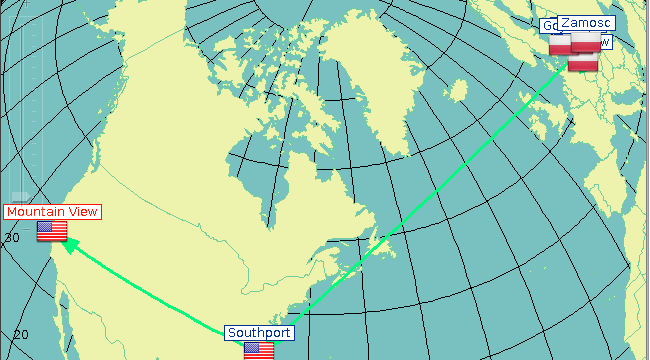
\includegraphics[width=\textwidth]{img2/google.png}
\centering google.com - amerykańska wyszukiwarka internetowa
 \\
\\
  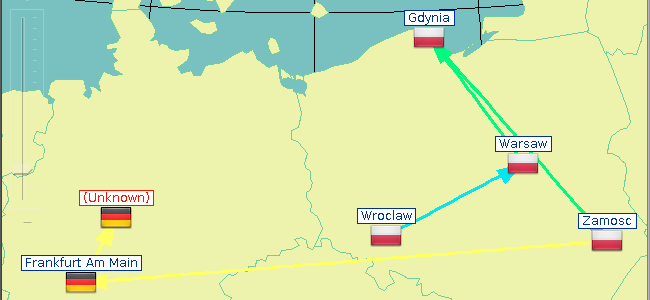
\includegraphics[width=\textwidth]{img2/wprost.png}
\centering wprost.pl - polski serwis informacyjny

\end{document}
